Пример моделирования: $m=100GeV, \delta m = 10^{-4} GeV$
\begin{columns}[c]
	\begin{column}{0.5\textwidth} % Left column width
		\begin{figure}
				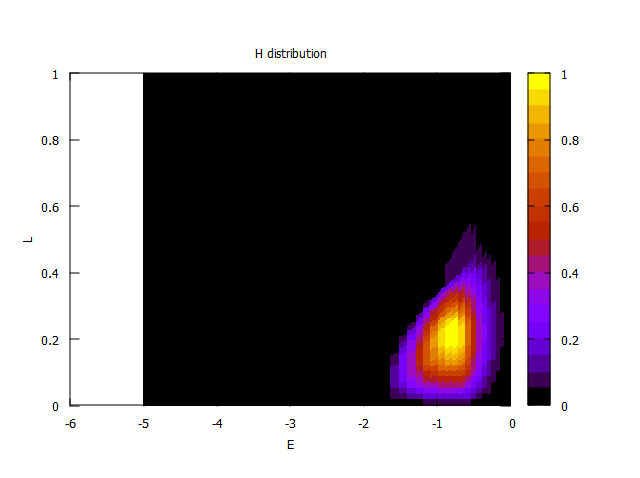
\includegraphics[width=\linewidth
				]{images/dh_100_dm.png}
				\caption{захват тяжелой компоненты}
		\end{figure}
	\end{column}
	\begin{column}{0.5\textwidth} 
		\begin{figure}
				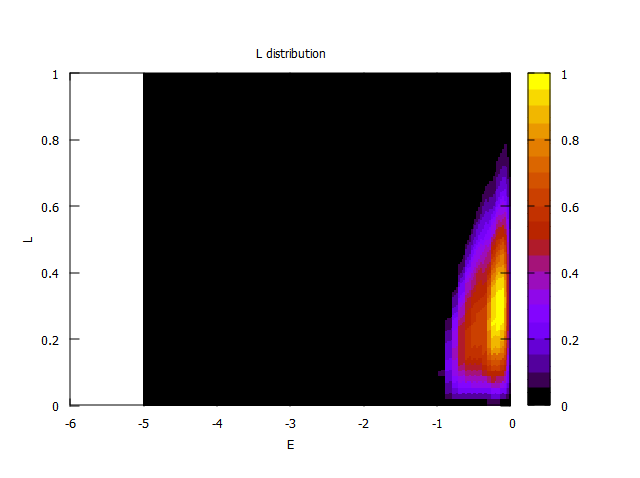
\includegraphics[width=\linewidth]
				{images/dl_100_dm.png}
				\caption{захват легкой компоненты}
		\end{figure}
	\end{column}
\end{columns}